\mysection{Collecting Data for Modelling the System}\label{data}

Before being able to build a system model, we must first collect some data about the application and the available resources.

\mysubsection{General Approach}

Quite little information is needed for constructing a system performance model, yet some data is fundamental for the following analysis.
What are the specifications of the incoming event streams, including their patterns, periods and deadlines?
Which of these events can occur in parallel?
(Note that this information needs to be given by formal specifications, not from observation or simulation~\cite{wan:06}.)
What resource demands do the tasks have?
How are the processing capacities and patterns of the available system resources specified?
What scheduling technique to use?

Here we can have very different degrees of detail, as sometimes we can design the new system pretty much freely, while other times we already got specific components and architectures to use given.
Yet, in case we can freely design the system, we can now just set these parameters arbitrarily and later on, for example in \autoref{sensitivityAnalyis}, optimize them.

\mysubsection{Sample System: A Simple Message Receiver} 
To illustrate the use of MPA we will design our own little embedded system.
First the requirements to this system have to be collected.
We want to construct a simple gadget that can receive messages via a signal.
Each of the messages consists out of one to 20 ASCII characters that are displayed to the device screen once the message got received.
Besides receiving messages, the device's user can also adjust the screen's brightness by pressing the ``brighter'' or the ``darker'' button.
Other functionalities will not be implemented, especially it will not be possible to compose or send any own messages.

Therefore, the system has only two use cases that can be described using UML sequence charts (see \autoref{fig:seq_brightness} and \autoref{fig:seq_message}).

\begin{figure}
    \centering
    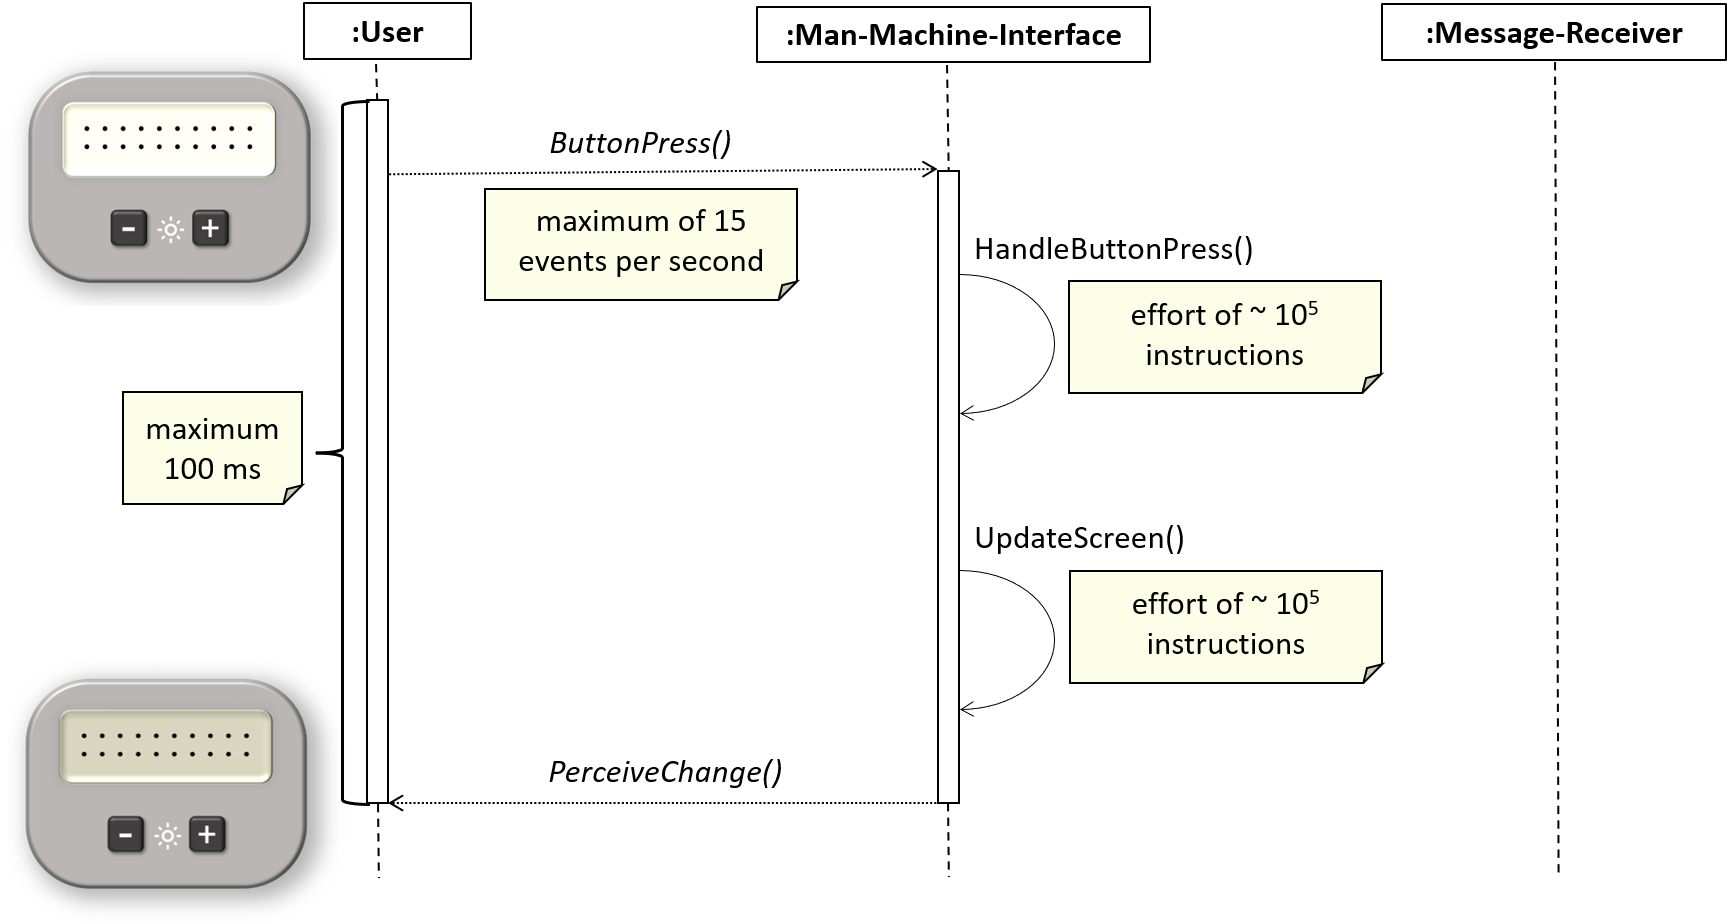
\includegraphics[width=\columnwidth]{graphics/sequence_brightness.png}
    \caption{Annotated UML Sequence Chart of the Use Case ``changing the screen's brightness''}\label{fig:seq_brightness}
\end{figure}

\begin{figure}
    \centering
    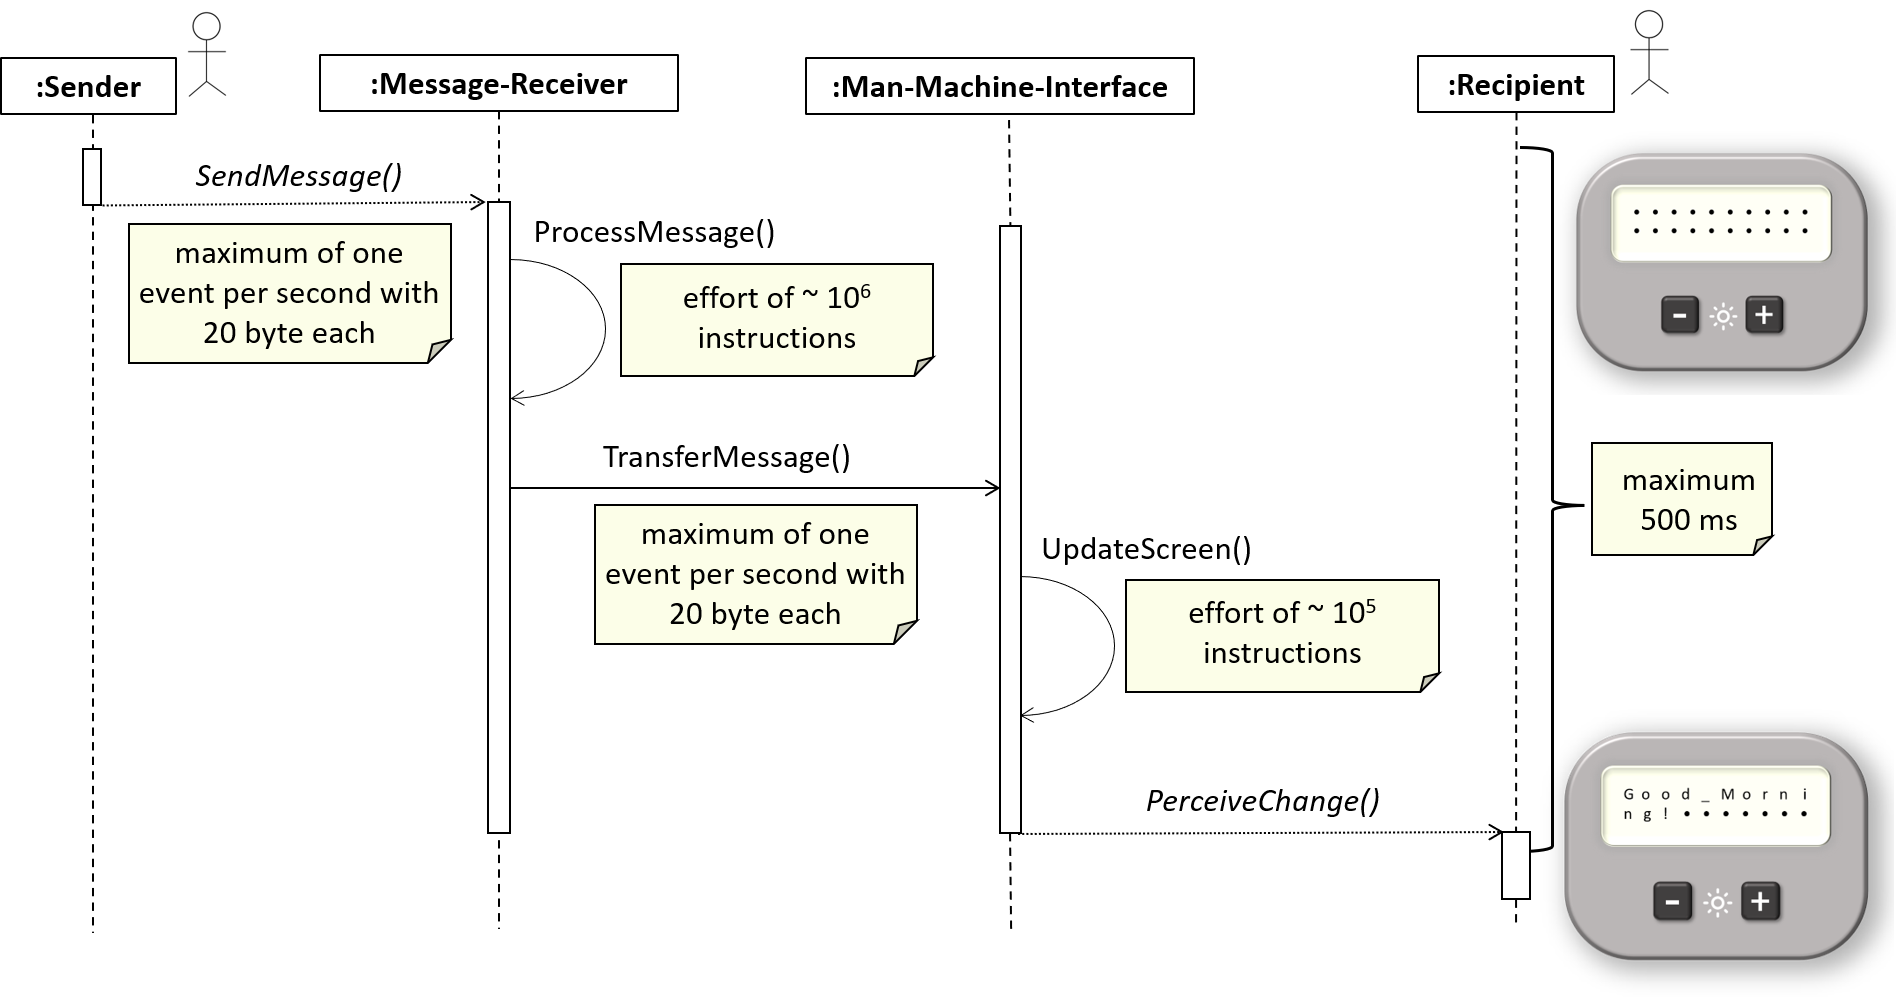
\includegraphics[width=\columnwidth]{graphics/sequence_message.png}
    \caption{Annotated UML Sequence Chart of the Use Case ``receiving a message''}\label{fig:seq_message}
\end{figure}
